% !TEX root = ../Poissons.tex

\section{Operadic diagonals}

\subsection{Cellular diagonals for polytopes}

The usual \emph{thin diagonal} of a topological space $X$ is the map $\Delta : X \to X \times X$ defined by $\Delta(x):=(x,x)$ for all $x \in X$.

\begin{definition}
    A \emph{cellular diagonal} of a polytope $P$ is a continuous map $P \to P \times P$ such that
    \begin{enumerate}
        \item its image is a union of $\dim P$-faces of $P\times P$ (i.e. it is \emph{cellular}),
        \item it agrees with the thin diagonal on the vertices of $P$, and
        \item it is homotopic to the thin diagonal, relative to the image of the vertices. 
    \end{enumerate}
    A cellular diagonal is said to be \emph{face-coherent} if its restriction to a face of $P$ is itself a cellular diagonal for that face. 
\end{definition}

A powerful geometric technique to define face-coherent cellular diagonals on polytopes first appeared in \cite{fultonIntersectionTheoryToric1997a}, was presented in \cite{masudaDiagonalAssociahedra2021}, and was fully developed in \cite{LA21}.
The key idea is the following: any vector $\vec v$ in generic position with respect to $P$ defines a cellular diagonal $\triangle_{(P,\vec v)}$, via the following formula
\begin{align*}
    \begin{array}{rlcl}
    \triangle_{(P,\vec v)}\  : & P &\to  &P\times P\\
    &z & \mapsto& 
    \bigl(\min_{\vec v}(P\cap \rho_z P),\,  \max_{\vec v}(P\cap \rho_z P)\bigr) \ .
    \end{array}
\end{align*}
Here, $\rho_z P := 2z-P$ denotes the reflection of $P$ with respect to the point $z$, and $\min_{\vec v}(P)$ denotes the unique vertex of $P$ which minimizes the scalar product with $\vec v$. 
The diagonal $\triangle_{(P,\vec v)}$ defines a canonical polytopal subdivision of $P$: it is by construction a tight coherent section of the projection $\pi : P \times P \to (P+P)/2$, and one just needs to draw the polytopes $(F+G)/2$, for all pairs of faces $(F,G) \in \Ima \triangle_{(P,\vec v)}$.
For the rest of the paper, every time we will speak about a diagonal, \emph{we will always mean such a map}. 

\begin{definition}
    \label{def:diagonal}
    A \emph{cellular diagonal} or simply a \emph{diagonal} $\triangle_{(P,\vec v)}$ of the permutahedron~$P$ is a tight coherent section of the projection $P \times P \to P, (x,y) \mapsto (x+y)/2$.
\end{definition}

Such a map can be seen as a topological map, or sometimes as a map of lattices; we shall not change notation and the context should make clear which 
We will sometimes denote a diagonal of the $n$-permutahedron by $\triangle_n$. 

\begin{definition}
    The \emph{$f$-vector} of the diagonal $\triangle_{(P,\vec v)}$ is the number of faces of $P\times P$ of given total dimension in its cellular image.
    Alternatively, it is the $f$-vector of the polytopal complex~$\pi (\triangle_{(P,\vec v)})$.
\end{definition}

For the purpose of studying this $f$-vector, one can study the dual of the polytopal complex.

\begin{proposition}
    The $f$-vector of a cellular diagonal of the permutahedron $\triangle_{(P,\vec v)}$ is given by the opposite of the $f$-vector of the hyperplane arrangement made of the braid arrangement together with a second copy of it, translated in the generic direction $\vec v$. 
\end{proposition}

\begin{proof}
    This follows from \cite[Proposition 1.3]{LA21}; \cite[Corollary 1.4]{LA21} describes precisely the intersection poset of this hyperplane arrangement.
\end{proof}
 
The first part of the paper provides explicit formulas for this $f$-vector. 

%%%%%%%%%%%%%%%%%%%%%%%%%%%%%%%%%%%%%%%%%%%%%%%%

\subsection{Cellular diagonals for the permutahedra}
\label{s:diagonals-permutahedra}

Let us first set up some notations that will be of use throughout the paper. 
A set $\sigma_I := \bigcup_{i\in I} \sigma_i$ is a \emph{partition} of $[n]:=\{1,\ldots,n\}$ if $\bigcup_{i\in I} \sigma_i = [n]$ and $\sigma_i \cap \sigma_j = \emptyset$ for $i \neq j$.
The subsets $\sigma_i$ are called \emph{blocks}. 
We denote by $|\sigma|:=|I|$ the size of the partition (its number of blocks).
A partition is \emph{ordered} if the indexing set $I$ is equipped with a total order; in what follows we shall use $I=[k]$ for $k \in \N$. 
We use the shorthand $14|23$ to denote both the unordered  partition $\{\{1,4\},\{2,3\}\}$, and also the ordered partition $(\{1,4\},\{2,3\})$ (when the order is clear from context).

\begin{figure}
	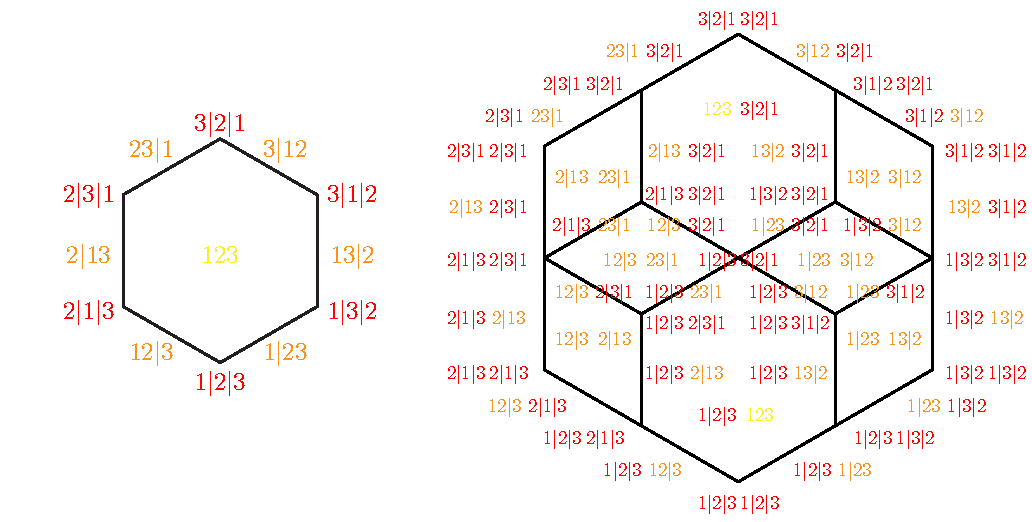
\includegraphics[scale=.9]{diagonalPermutahedron2}
	\caption{Labelings of the faces of the permutahedron~$\Perm[3]$ by ordered partitions of~$[3]$ (left) and of the faces of the LA diagonal  $\LAD$ of the permutahedron~$\Perm[3]$ by pairs of compatible ordered partitions of~$[3]$ (right).}
	\label{fig:diagonalPermutahedron2}
\end{figure}
\vincent{I have included this picture here to be sure that we don't forget it. I should make one for the SU diagonal~$\SUD$ as well.}

Let us recall the combinatorial formula for the cellular approximation of the diagonal of the permutahedra from \cite[Theorem 3.16]{LA21}.
Let $n\geq 1$, and let us write \[ \LA(n) \coloneqq \{(I,J) \ | \ I,J\subset\{1,\ldots,n\}, |I|=|J|, I\cap J=\emptyset, \min(I\cup J)\in I \}. \] 
Let $\vec v \in \R^n$ be such that $\forall (I,J) \in \LA(n)$, we have $\sum_{i \in I} v_i > \sum_{j \in J} v_j$, and let $P\subset \R^n$ denote the standard $(n-1)$-dimensional permutahedron.
For any pair $(\sigma,\tau)$ of ordered partitions of $[n]$, we have
\begin{eqnarray*}
    (\sigma,\tau)\in \Ima\triangle_{(P,\vec v)} 
    & \iff & \forall (I,J) \in \LA(n), \exists k \in [n] , 
    \left| \sigma_{[k]} \cap I \right|
    >
    \left| \sigma_{[k]} \cap J \right| \text{ or } \\
    && \exists l \in [n] , 
    \left| \tau_{[l]} \cap I \right|
    <
    \left| \tau_{[l]} \cap J \right|  \ . 
\end{eqnarray*}
We shall denote by $\LAD$ the set of pairs of ordered partitions of $[n]$ which satisfy the above condition. 
There is an equivalent description of $\LAD$ which has the following form: 
\begin{proposition}
\label{p:minimal}
For a two ordered partitions $\sigma, \tau \subset [n]$, we have
\begin{eqnarray*}
    (\sigma,\tau)\in \LAD 
    & \iff & \forall (I,J) \in \LA(\sigma,\tau), \exists k \in [n] , 
    \left| \sigma_{[k]} \cap I \right|
    >
    \left| \sigma_{[k]} \cap J \right| \text{ or } \\
    && \exists l \in [n] , 
    \left| \tau_{[l]} \cap I \right|
    <
    \left| \tau_{[l]} \cap J \right|  \ . 
\end{eqnarray*}
\end{proposition}
Here, $\LA(\sigma,\tau) \subset \LA(n)$ is a proper subset of $\LA(n)$ which depends on the choice of~$(\sigma,\tau)$, and comes from the geometry of the situation, see \cite[Theorem 1.26]{LA21} for more details.
For our present purposes, it will be enough to restrict our attention to facets of $\LA$, that is pairs $(\sigma,\tau)$ which satisfy $|\sigma| + |\tau|=n+1$.
In this case, $\LA(\sigma,\tau)$ has $n-1$ elements, and admits the following description. 

For any subset $\sigma_i \subset [n]$, let $\vec \sigma_i \in \R^n$ denote the boolean vector whose coordinates are given by $1$ in position $j$ if $j \in \sigma_i$ and $0$ otherwise. 
Given a facet $(\sigma,\tau)$ of $\LAD$, one can consider the system of equations $\langle \vec \sigma_i , x \rangle=0$, $\langle \vec \tau_j , x \rangle=0$ given by the blocks of both partitions.
For geometric reasons (see the proof of \cite[Theorem 1.26]{LA21}), the solution of this system is $x=0$. 
Now we will be interested in the solutions of the systems associated to the pairs $(\sigma',\tau)$ and $(\sigma,\tau')$ where $\sigma'$ (resp. $\tau'$) has been obtained from $\sigma$ (resp. $\tau$) by merging two adjacent blocks.

\begin{proposition}
\label{p:minimal-IJ-pairs}
    There is a bijection between the set $\LA(\sigma,\tau)$ and the solutions to the systems of equations of the form $(\sigma',\tau)$ and $(\sigma,\tau')$. 
\end{proposition}

\Guillaume{A revoir!! Il faut utiliser le fait que ce sont des facettes!!}

\begin{proof}
    For any $z \in (\mathring \sigma+ \mathring \tau)/2$, the face $\tau \cap \rho_z \sigma$ of $P \cap \rho_z P$ is a vertex of the polytope $P \cap \rho_z P$.
    The faces of the form $\tau \cap \rho_z \sigma'$ and $\tau' \cap \rho_z \sigma$ are the edges of $P\cap \rho_z P$ which are adjacent to the vertex $\tau \cap \rho_z \sigma$. 
    By definition $D(\sigma, \tau)$ describes the directions of these edges, and the translation is made as follows: for a given pair $(I,J)$, define the corresponding direction $\vec d$ by its coordinates $d_i:=1$ if $i \in I$, $d_j:=-1$ if $j \in J$, and $d_k:=0$ otherwise.  
    We refer to \cite[Section 1.5]{LA21} for more details.
\end{proof}

We will sometimes refer to the elements of $\LA(\sigma,\tau)$ as the \emph{minimal $(I,J)$-pairs}.



